\chapter{Memory Layout, Relocation, and Executable Images}
\label{ch:link-layout}

Resolving \code{answer} to a definition tells the linker which bytes implement the function.
It does not yet tell the caller where those bytes will live.
Layout assigns addresses subject to alignment, ordering, capacity, and permission constraints; relocation then turns symbolic relationships into field values at those addresses.
A linker that applies relocations before its last layout change writes stale addresses.
A linker that treats a file offset as a virtual address can produce an internally consistent file that fails immediately when loaded.

This chapter uses the two-object demo to compute the whole image, including padding and zero-fill.
It also explains why script languages are policy interfaces rather than replacements for arithmetic validation.
ELF program headers define the loader-facing contract, while the linker script determines how input sections are arranged to satisfy it~\cite{xinuos-2026-elf,gnu-2026-ld}.

\section{Keep three coordinate systems separate}
\label{sec:ch58-coordinates}

An input symbol starts with an offset in its defining input section.
Placement assigns that input section a position within an output allocation.
The allocation has a virtual address in the eventual process image.
For an ordinary defined symbol,
\[
 S=B_r+O_{input}+V_{symbol},
\]
where $B_r$ is the region base, $O_{input}$ the input section's placement within the region, and $V_{symbol}$ its section-relative value.
An absolute symbol is the exception: it retains its recorded value.

File offsets are a fourth useful quantity, but not another term in that address equation.
They locate serialized bytes in the executable file.
The program headers relate file offsets to virtual addresses for each segment.
A file offset of \code{0x1000} can describe code loaded at \code{0x401000}; adding the file offset to a symbol's section offset does not produce its runtime address.
Figure~\ref{fig:ch58-coordinates} follows the helper's three address components.

\begin{figure}[htbp]
\centering
\begin{tikzpicture}[node distance=14mm]
\node[basic block] (v) {answer in answer.o: offset 0};
\node[basic block,below=of v] (o) {answer.o text placed at region +32};
\node[basic block,below=of o] (b) {code region base: 0x401000};
\node[basic block,below=of b] (s) {answer address: 0x401020};
\draw[cfg edge] (v)--(o); \draw[cfg edge] (o)--(b); \draw[cfg edge] (b)--(s);
\end{tikzpicture}
\caption{A symbol's final address combines its input offset with placement and region base, not with its file offset.}
\label{fig:ch58-coordinates}
\end{figure}

\section{Alignment is checked arithmetic}
\label{sec:ch58-alignment}

For a nonzero power-of-two alignment $a$, rounding $x$ upward can be written
\[
 \operatorname{alignup}(x,a)=(x+a-1)\mathbin{\&}\mathop{\sim}(a-1).
\]
That machine expression is valid only after checking the alignment's form and proving that $x+a-1$ does not overflow.
The mathematical intent is the smallest multiple of $a$ at least $x$.
An implementation using an overflowing intermediate can wrap a large requested address back into a small region and defeat a later bounds check.

Input sections carry alignment requirements, and placement rules can impose stricter ones.
For power-of-two alignments, taking their maximum satisfies both.
If arbitrary alignment values were permitted, the maximum would not generally be enough; their least common multiple would express the combined requirement.
The case study accepts only powers of two through 4096, making the maximum rule explicit and correct.

\begin{algorithm}[htbp]
\caption{Place one input section in a bounded region.}
\label{alg:ch58-place}
\begin{pseudocode}
\Require region base $B$, capacity $C$, used extent $u$, section size $n$, alignments
\Ensure aligned nonoverlapping placement inside the region, or a diagnostic
\State $a\gets\max(inputAlignment,ruleAlignment)$; validate supported power of two
\State $v\gets\operatorname{checkedAlignUp}(B+u,a)$
\State $o\gets v-B$
\State require $o\le C$ and $n\le C-o$
\State record input section address $v$ and region offset $o$
\If{$n>0$}
  \State update used extent to $o+n$
\EndIf
\end{pseudocode}
\end{algorithm}

Algorithm~\ref{alg:ch58-place} uses subtraction-based capacity checking to avoid computing an unchecked endpoint.
With prevalidated region endpoints, each placement is constant-time apart from copying initialized bytes.
A sequential placement policy is deterministic but is not a general bin-packing optimizer.
If the requested order exceeds a region, the linker reports the overflow rather than silently moving contributions into a different region with different semantics.

\section{Compute the demo layout completely}
\label{sec:ch58-demo}

The Lua map defines code at \code{0x401000} and data at \code{0x406000}, each with a 16 KiB capacity.
Text contributions are placed in input-object order with alignment 16.
The first text contribution is 31 bytes, so the second begins at offset 32 after one padding byte.
The second contributes six bytes.
Table~\ref{tab:ch58-layout} computes all nonempty input placements.

\begin{table}[htbp]
\caption{The two objects occupy separate input ranges inside the mapped code and data regions.}
\label{tab:ch58-layout}
\centering
\begin{tabular}{llll}
\toprule
Input contribution & Size & Alignment used & Virtual start \\
\midrule
demo.o text & $31$ & $16$ & \code{0x401000} \\
answer.o text & $6$ & $16$ & \code{0x401020} \\
demo.o data & $8$ & $8$ & \code{0x406000} \\
demo.o BSS & $32$ & $16$ & \code{0x406010} \\
\bottomrule
\end{tabular}
\end{table}

The code memory extent is $32+6=38$ bytes.
The data region contains eight initialized bytes, eight alignment bytes before BSS, and 32 bytes of BSS, giving 48 bytes of memory extent.
Because the alignment gap and BSS are both zero-initialized tail storage, only eight data payload bytes need appear in the executable file.
Figure~\ref{fig:ch58-data} shows the resulting distinction between \code{p\_filesz} and \code{p\_memsz}.

\begin{figure}[htbp]
\centering
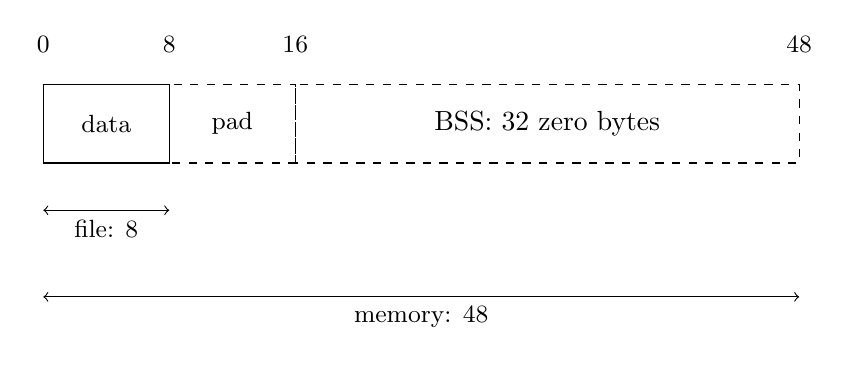
\begin{tikzpicture}[x=2mm,y=10mm]
\draw (0,0) rectangle (8,1); \node[font=\small] at (4,0.5) {data};
\draw[dashed] (8,0) rectangle (16,1); \node[font=\small] at (12,0.5) {pad};
\draw[dashed] (16,0) rectangle (48,1); \node at (32,0.5) {BSS: 32 zero bytes};
\draw[<->] (0,-0.6)--node[below,font=\small] {file: 8}(8,-0.6);
\draw[<->] (0,-1.7)--node[below,font=\small] {memory: 48}(48,-1.7);
\foreach \x in {0,8,16,48} \node[font=\small] at (\x,1.5) {\x};
\end{tikzpicture}
\caption{The loader supplies the zero tail, including alignment before BSS, without reading forty additional payload bytes.}
\label{fig:ch58-data}
\end{figure}

If initialized bytes followed the NOBITS contribution in the same segment, a simple initialized-prefix/zero-tail representation would no longer suffice without materializing a gap or creating another segment.
Our linker rejects that ordering.
This restriction is narrower than ELF itself but keeps the chosen segment representation unambiguous.
Zero-sized sections receive identities when mapped but do not advance the occupied extent merely to satisfy an otherwise unused alignment boundary.

\section{Patch relocations from final identities and addresses}
\label{sec:ch58-patch}

After layout, the chosen definition of \code{answer} has address \code{0x401020}.
The external call field is at \code{0x401012}, and its addend is $-4$.
The value is therefore \code{0x401020 - 4 - 0x401012 = 0x0A}.
The loop branch field at \code{0x40100D} targets \code{0x401005}, giving $-12$.
The initialized data pointer receives the full address \code{0x401020}.
Table~\ref{tab:ch58-patches} records both arithmetic and bytes.

\begin{table}[htbp]
\caption{Final relocation values are checked independently of the emitted program's exit status.}
\label{tab:ch58-patches}
\centering
\begin{tabular}{lll}
\toprule
Field & Numeric result & Little-endian bytes \\
\midrule
Loop PC32 & $-12$ & \code{F4 FF FF FF} \\
Call PC32 & $10$ & \code{0A 00 00 00} \\
Answer pointer & \code{0x401020} & \code{20 10 40 00 00 00 00 00} \\
\bottomrule
\end{tabular}
\end{table}

\begin{algorithm}[htbp]
\caption{Apply one relocation only after validating its object-level and arithmetic contracts.}
\label{alg:ch58-relocate}
\begin{pseudocode}
\Require final placements, selected symbol definitions, one relocation record
\Ensure the designated field is patched with a representable target-specific value
\State validate target section, symbol index, relocation kind, and explicit addend
\State determine field width from relocation kind
\State require offset within target and width no larger than remaining payload
\State reject overlapping fields under the case-study object contract
\State compute symbol address $S$ and field address $P$
\State compute the relocation formula using defined checked arithmetic
\State enforce the relocation kind's signed or unsigned range rule
\State write exactly the field width in target byte order
\end{pseudocode}
\end{algorithm}

Algorithm~\ref{alg:ch58-relocate} separates object validation from numeric range checking.
A value that fits four bytes is still invalid if its field lies beyond the section payload.
Likewise, a valid field does not justify using an out-of-range symbol-table index.
The case study rejects overlapping relocation fields because it does not implement a composed-relocation protocol.
That is a supported-format restriction rather than a claim that every ABI forbids all relocation composition.

\section{Create program headers for the loader}
\label{sec:ch58-segments}

A section describes a link-time unit; a \code{PT\_LOAD} program header describes a runtime mapping.
Our linker emits one loadable segment per nonempty Lua region.
It writes them in increasing virtual-address order, independently of the order in which the Lua table declared the regions.
Each segment's file offset and virtual address are congruent modulo the 4096-byte page alignment.
The data memory size is at least its file size, and the entry address lies inside an executable input contribution~\cite{xinuos-2026-elf}.

Table~\ref{tab:ch58-segments} gives the demo's program-header values.
The file starts with headers; the first payload is padded to file offset \code{0x1000}.
The next payload is padded to \code{0x2000}.
The implementation also emits a non-executable GNU stack descriptor.
It does not emit a dynamic section, interpreter path, or runtime symbol table.

\begin{table}[htbp]
\caption{The demo's loadable segments map initialized prefixes and zero-filled tails at explicit virtual addresses.}
\label{tab:ch58-segments}
\centering
\begin{tabular}{llllll}
\toprule
Segment & File offset & Virtual base & File size & Memory size & Flags \\
\midrule
Code & \code{0x1000} & \code{0x401000} & $38$ & $38$ & R, X \\
Data & \code{0x2000} & \code{0x406000} & $8$ & $48$ & R, W \\
\bottomrule
\end{tabular}
\end{table}

The output intentionally has no section-header table.
The Linux loader uses the program headers, so the syscall-only demonstration can execute without retaining link-time sections.
This does not make the output a general-purpose C runtime image: the case study supplies no startup library, dynamic loader handshake, unwind metadata, or general auxiliary-vector consumer.
Its supported execution contract is the tested freestanding syscall program.

\section{Memory maps are policy, not permission to skip validation}
\label{sec:ch58-policy}

The Lua map returns an entry name, an ordered region array, and an ordered section-rule array.
Regions declare origins, capacities, and allowed permissions.
Rules match exact input-section names and select their region and minimum alignment.
The host copies these declarations into its own representation before placement.
It then checks duplicate names, unknown regions, overlap, alignment, permission compatibility, and capacity.

The use of Lua does not imply that any numeric Lua value is a valid address.
Lua 5.4 distinguishes integers from floating-point numbers; the host requires nonnegative integer values for origins, lengths, and alignments~\cite{ierusalimschy-2026-lua}.
A floating-point value can lose low address bits before the linker sees it.
An overflowing Lua integer calculation can wrap before validation, so the script author must express intended arithmetic carefully and the host still validates the resulting range.
It cannot reconstruct an intention already lost inside an arbitrary script calculation.

Figure~\ref{fig:ch58-policy} shows the division of responsibility.
The script chooses a layout policy; the host proves the selected input contributions fit that policy before modifying relocation fields.
A production script language often adds wildcard matching, computed symbols, and assertions over final sizes.
Each addition creates evaluation-order and dependency questions that need an explicit contract.

\begin{figure}[htbp]
\centering
\begin{tikzpicture}[node distance=15mm]
\node[basic block] (lua) {Lua: choose regions and ordered rules};
\node[basic block,below=of lua] (validate) {C: validate and place all contributions};
\node[basic block,below=of validate] (patch) {C: resolve final addresses and patch fields};
\draw[cfg edge] (lua)--node[right,font=\small] {copied policy}(validate);
\draw[cfg edge] (validate)--node[right,font=\small] {checked layout}(patch);
\end{tikzpicture}
\caption{Executable configuration proposes placement; the linker retains responsibility for the resulting image invariants.}
\label{fig:ch58-policy}
\end{figure}

\section{Embedded images distinguish load and run addresses}
\label{sec:ch58-lma}

A program for a microcontroller may store initialized writable data in flash but execute with that data in RAM.
The load memory address identifies where the initial bytes reside in the image; the virtual or run address identifies where instructions expect the object during execution.
Startup code copies the initialization image and clears BSS before ordinary language-level code runs.
A linker can emit copy-table symbols or records to describe those operations.

For example, 12 initialized bytes stored at flash address \code{0x100080} might run at RAM address \code{0x200010}.
An absolute pointer to a variable four bytes into that data refers to \code{0x200014}, not \code{0x100084}.
The startup copy reads the latter location and writes the former.
GNU linker scripts expose load/run address distinctions explicitly~\cite{gnu-2026-ld}.
The present x86-64 Linux case study does not implement separate load/run addresses; its region addresses are process virtual addresses.

\section{Changing layout after relocation requires another proof}
\label{sec:ch58-relayout}

Thunk insertion, relaxation, section garbage collection, and identical-code folding can change the addresses used by relocations.
Their phase order must therefore preserve or recompute all affected addresses and fields.
One safe organization chooses transformations, recomputes layout, and only then applies final relocations.
When transformations themselves depend on distances, the linker needs an iteration strategy with a termination argument and a final range check.

A veneer can make an otherwise out-of-range branch reachable by introducing an intermediate target, but its own addressing sequence and placement also have range and ABI constraints.
It is not a universal instruction-independent repair for every overflowing relocation.
Our implementation reports range overflow instead of synthesizing thunks.
Tests place a target beyond the PC32 range and verify an error, and separately exercise exact signed-32 endpoints by controlling a relocation addend.
Acceptance at the two endpoints and rejection immediately beyond them checks the signedness of the range predicate directly.

\section{Exercises}
\label{sec:ch58-exercises}
\begin{enumerate}
\item\label{ex:ch58-layout} Replace the first text contribution by 47 bytes while retaining alignment 16 and a six-byte second contribution. Compute the second start and code extent.
\item\label{ex:ch58-zero} Increase BSS alignment from 16 to 32 in the demo. Compute data memory size and the number of zero-supplied bytes.
\item\label{ex:ch58-rebase} Move the entire code region by \code{0x200000} while preserving internal order. Which two PC-relative fields stay unchanged, and what happens to the absolute pointer?
\item\label{ex:ch58-file} Explain why file offset \code{0x2000} is not the runtime address of the initialized pointer in Table~\ref{tab:ch58-segments}.
\item\label{ex:ch58-lma} For the flash/RAM example, give the source and destination addresses of the fifth byte copied and the address a program pointer to that byte must contain.
\end{enumerate}

\section{Further reading}
\label{sec:ch58-reading}
ELF program-header rules define file/memory sizes, permissions, alignment congruence, and segment ordering~\cite{xinuos-2026-elf}.
GNU linker documentation develops memory regions, section placement, load addresses, and script expressions~\cite{gnu-2026-ld}.
The AMD64 supplement defines the relocation arithmetic applied after those placements~\cite{matz-2012-amd64}.
